
\documentclass[12pt,a4paper]{mcmthesis}
\usepackage{ctex}
\usepackage{lipsum}
\usepackage{graphicx}
\usepackage{booktabs,colortbl}
\usepackage{xcolor}
\usepackage{tikz}
\usepackage{indentfirst}
\mcmsetup{CTeX = true,
        tcn ={\xiaowuhao 202105135237 }, problem = A,
        sheet = true, titleinsheet = false, keywordsinsheet = true,
        titlepage = true, abstract = true}
\usepackage{newtxtext}
\usepackage{lipsum}
\usepackage{cite}
\usepackage{amsmath}
\usepackage{paralist}
\let\itemize\compactitem
\let\enditemize\endcompactitem
\let\enumerate\compactenum
\let\endenumerate\endcompactenum
\let\description\compactdesc
\let\enddescription\endcompactdesc

\setlength\abovedisplayskip{5pt}
\setlength\belowdisplayskip{-8pt}
\setlength{\parskip}{0.1em}

\newcommand\wordc[1]{\textbf{#1}}
\renewcommand{\appendixtocname}{附\quad录}
\renewcommand{\appendices}{\hspace{-2em}{\sanhao\HEI {\bf 附~~~录}}}
\colorlet{tableheadcolor}{gray!25} % Table header colour = 25% gray
\newcommand{\headcol}{\rowcolor{tableheadcolor}}

\title{\textcolor{red}{数学建模竞赛论文的题目(三号黑体)}}
\date{}

\usepackage{zhnumber} % change section number to chinese
\renewcommand\thesection{\zhnum{section}、\hspace{-1em}}
\renewcommand\thesubsection{\arabic{section}.\arabic{subsection}}

\usepackage[T1]{fontenc}
\usepackage[utf8]{inputenc}
\usepackage[font=small,labelfont={bf,sf},tableposition=top]{caption}

\makeatletter
   \renewcommand{\thefigure}{\ifnum \c@section>\z@ \arabic{section}-\fi \@arabic\c@figure}
   \renewcommand{\thetable}{\ifnum \c@section>\z@ \arabic{section}-\fi \@arabic\c@table}
\makeatother

\begin{document}
\begin{abstract}
%abstract---------------
    {\song\xiaosihao
\setlength{\parindent}{2em}{轨道交通影响一个城市的运转效率。呼和浩特市在2019年建成地铁并投入使用,然而地铁的建设和维护需要消耗大量的财力和物力,需要考虑车厢节数、发车间隔、新站点选址这些指标,使其达到成本尽可能小,而乘客体验更优。所以我们就从这几个变量入手,进行优化模型的建立。}


\setlength{\parindent}{2em}{在第一个问题中,我们首先使用混合高斯模型对地铁客流量数据进行仿真,通过Fisher聚类方法对地铁运营的高峰、低峰时段进行划分。通过构建目标函数,加以条件限制得到4-6节车厢编组的建议,并给出了详细的发车时间间隔表。}

\setlength{\parindent}{2em}第二问,依据该市热点图和拥堵路段,确定需要改进的路段。采用最小二乘估计进行建模,之后对找到重点节点,对重点区域进行加权最小二乘估计的建模,拟合出所需的路线。对于地铁盈利的确定则是考虑影响成本的主要条件,加以限制,用优化模型解决。

\setlength{\parindent}{2em}第三问基于高峰情况发生的背后原因以及错峰出行的实质意义,建立优化模型,利用算法求得结果,输出出行时间与目的节点对应表格。为疫情防控提出切实可行的方案。

\setlength{\parindent}{2em}第四问在综合考虑公交地铁互补出行以及现有快速路的分布下,给出了公交线路规划方案以及一些注意事项。

\setlength{\parindent}{2em}最后对于模型的部分闲置进行总结和反思,总结了局限性和展望。
}


\begin{keywords}
{\song\xiaosihao
\textcolor{red}{使用到的模型名称、方法名称、特别是亮点一定要在关键字里出现,3$\sim$ 5个较合适。}}
\end{keywords}

\begin{itemize}
  \item \textcolor{blue}{前面一页必须使用模板格式(黑色部分),否则论文检测不通过。}
  \item \textcolor{blue}{此页为论文开始处,论文正文用阿拉伯数字从“1”开始连续编号,页码位于每页页脚中部。(目录可加可不加)}
\end{itemize}

\end{abstract}
\maketitle
\renewcommand{\contentsname}{\centerline{\sanhao\bfseries\HEI 目\quad 录}}
%\thispagestyle{empty}
%{\song\xiaosihao
\tableofcontents
%}

\newpage
\setcounter{page}{1}
\section{问题重述}
\subsection{引言}
%Introduction---------------

\setlength{\parindent}{2em}
{呼和浩特市地处中国的华北地区、北部地区,建成区面积约为260平方千米,常住人口在344万左右。截止2020年10月,呼和浩特市已经开通运营路线2条,地铁里程总长约49千米,车站总计43站。}

{在工作日,地铁通常用于满足人们通勤的需求,这样符合地铁建设的初衷,缓解交通高峰时段的交通拥堵。呼和浩特市的城市总面积较大,但常住人口相对较少,人口基数小,会直接应该影响地铁的当日客流量,从而直接影响运营的成本。}

{本文的目的就是想从车厢数量和发车间隔的确定入手,继而进行新增地铁线路的选址,并尽可能保证地铁可以营利。最后要基于地铁和公交现状,提出新的地铁和公交互补的公交线路,普惠于呼和浩特人民。}


\subsection{要解决的具体问题}

   1.当前的地铁运营是否合理?
   
   \begin{table}
  	\centering
  	\begin{tabular}{|l|l|l|}
  		\hline
  		& 早高峰 & 晚高峰 \\ \hline
  		工作日 & 7:00-9:00 & 17:00-19:00 \\ \hline
  		节假日 & 9:00-11:00 & 16:00-18:00 \\ \hline
  	\end{tabular}
  	\caption{早晚高峰时间表} 
  	\label{tab:早晚高峰}
  \end{table}
  呼和浩特市地铁运营时间为6:00-22:00,地铁型号为6B,每一列地铁最多容纳6*400人次。目前实行错峰发车,具体信息如 \ref{tab:早晚高峰}所示。在高峰发车间隔6分钟,在平峰时刻发车间隔10分钟,在晚20点以后发车间隔为12分钟。尽管在官方报道的客流量数据中,地铁客流量在逐渐增加,2020年12月6日,地铁客运量达到了17万人次,但是每天单向会发出100次,粗略的平均每列地铁的人次在400左右,载客率过低,也导致亏损十分严重。同时发车间隔也是影响成本的重要指标,在高峰时期的发车间隔短,可以优化乘客的乘车体验。在平峰和低峰时期,减少发车的次数,尽管会在一定程度上影响乘客的出行,但更大程度上会减少运营成本。所以我们需要先对当下的运营情况进行评估,然后给出最优车厢数量和发车间隔

  
  {2.建设新的线路选址在哪里?}
  
  {在新建新的线路的过程中,我们需要选择新的地点,来确保更多人会选择地铁这种运行方式,并且需要预测出每天至少需要多少人,才能满足地铁盈利的需求。}
 
  {3.实现学生党和工作党的错峰出行,实现平峰目标该怎么做?}
  
   {考虑到疫情的特殊背景,我们需要对不同站点的学生和工作者进行出行时间设定,以满足疫情防控的需要}
  
  {4.如何对公交新增线路,实现地铁公交更好的互补?}
  
   {将公交和地铁结合,通过相互补充满足更多人员高峰出行的需求。}
  
  {一些都可以用的东西。轨道交通影响整个城市的运转效率,发车间隔对整个轨道系统影响至关重要。运营公司自然希望在满足客流需求的太欧剑侠获得最大的收益,尽可能提升列车周转量与满载率。}
  {假设到站乘客服从均匀分布}



\section{名词解释与符号说明}

\subsection{名词解释与说明}
\begin{enumerate}
	\item \wordc{断面客流量:}在单位时间内,沿同一方向通过对到交通线路某断面你的乘客数量,即通过该断面你所在区间的客流量,分为上行断面客流量。
	
	\item \wordc{最大断面客流量:}在单位时间内,通过轨道交通线路各断面的客流量的最大值。
	
	\item \wordc{满载率:}反应车辆乘客满载程度的相对值,衡量车量利用程度的指标,可通过实际载客量与额定载客量之比求得。
	
	\item \wordc{乘客到达率:}乘客在某单位时刻在某一站点下车人数,单位通常为人/min。
	

	
	
\end{enumerate}
\subsection{主要符号与说明}

%tab1
\begin{table}[h!]
	\centering
	\small
	\begin{tabular}{p{60pt}<{\centering}|p{60pt}<{\centering}p{180pt}<{\raggedright}}
		\hline
		\headcol 序号 & 符号 & 符号说明 \\
		\hline
		1 & $M$ & 地铁车站的总数量 \\
		2 & $N$ & 当日的发车次数\\
		3 & $t_{i}^{j}$ & 第i辆地铁到达第j个站点的时间\\
		4 & $\Delta {t_i^j}$ & $t_{i-1}^{j}$到$t_i^j$的时间间隔\\
		5 & $F(\Delta {t_i^j})$ & 在$\Delta t_i^j$时间间隔内的进站人数\\
		6 & $f_j(t)$ & 站点j的乘客到达率函数 \\
		7 & ${f(t)}$ & 地铁线路的乘客到达率\\
		8 & $\Delta(t)$ & 发车间隔 \\
		9 & $\overline{F}$ & 地铁的最大荷载人数 \\
		10 & $\eta_i$ & 第i量车辆的载客率\\
		11 & $W_i$ & 乘客要乘第i量车的等待时间 \\
		12 & $K$ & k取值为1-43,一号线二号线依次编号,1a为1,1t为20,2a为1... \\
		13 & $\Omega$ & 所有站点指标的集合,如1a、2u。 \\
		$\cdots$ & $\cdots$\\
		\hline
	\end{tabular}
	%\caption{符号与说明}
	\label{symbol}
\end{table}



\section{问题分析}

本次比赛的四个问题,本质上也都是在围绕一个核心的意义-如何让地铁运营方的收益和乘客的体验感同时可以到达一个更好的水平,也就是如何更好的“以乘客为本,兼顾效益”。

从乘客的角度,影响体验感的变量会有:平均等待时长、票价、地铁空间体验感等等。从运营者角度需要考虑的问题就是:发车间隔、站点选址、票价定价、运营成本。


\subsection{数据分析}
\begin{figure}[h!t]
	\centerline{\includegraphics[scale=0.4]{发车时间图}\quad
	}
	\caption{\song\wuhao
		发车时间图}
	\label{fig:发车时间图}
\end{figure}

附件一给出了每一个地铁站的经纬度坐标,容易发现,一号线共有20个站点,二号线共有24个站点,二号线的交点为新华广场站,在一号线中标号为$1h$,在二号线中标记为$2k$,地铁一号线的总运行时间在45分钟,二号线的总运行时间在47分钟。同时根据当前的发车时间间隔数据,可以求出发车时间表,如下图\ref{fig:发车时间图}

附件二中给出了在9月1日到9月14日共计14天的,自早上6点到晚上22点45分的各站点进出站的数据。数据间隔为15分钟,以9月1日6点的1A为例,进站数据为62人,即在6点到6点15期间有62人刷卡进站。由于具体时点的人员分布对于解决问题来讲没有那么重要,所以在每一个15分钟我们都认为,乘客的到达服从均匀分布,在上例中,就是每分钟约有4人进站。同时我们也认为乘客的等待时间服从均匀分布,如果是在非高峰期,那么就是服从均值为5,取值在[0,10]的均匀分布,如果在高峰期就是均值为3,取值为[0,6]的均匀分布。

此处的附件二给出了某一时点的进站数据和出站数据,对于进站的人员来说,既可以在两个地铁方向中选择一个方向(如果是中转站,就是4个方向),又可以在众多站点中选择一个终点,由于目前我们的数据无法获得,但此处依旧想引入一个转移矩阵的概念,前面定义了K,并且用数字代替了站名,用1代表1a,此处我们用$\Omega$代表所有点,其中$\Omega={1a,1b,1c...,2v,2w,2x}$表示所有站点的集合。我们设转移矩阵为X,其中$X_{ij}$表示从i个站点出发,到j个站点下车的概率。比如说,$X_{1a1k}$是指从伊利健康谷上车,从艺术学院下车的概率。这个概率的计算需要用到当日各闸机数据,通过整理所有路线的人次,用$\frac{单线程客流量}{总线路客流量}$即可获得一个转移概率矩阵,这一矩阵可以更明显的看出热点线路和热点区域。从而可以对某一站点的进站人员的大概率经过的行程进行估计。而本题中所给的数据,我们简单认为,进站人数中,以0.5的概率向两个方向行进。


\subsection{地铁客流随时间的分布研究}
\begin{figure}[h!t]
	\centerline{\includegraphics[scale=0.4]{客流图}\quad
	}
	\caption{\song\wuhao
		客流量图}
	\label{fig:客流量}
\end{figure}


我们将附件2的数据进行简要的处理,通过求和求出每个时间节点的总进站人数与总出站人数,得到了如下所示的图\ref{fig:客流量}。

在图中,橙色的线表示的是出站的数据,蓝色的是进站的数据,在发车的前一个半小时,我们进站数据比出站数据大,这是合情合理的,但是随着时间的推移,到14:15点附近时,会发现橙色的线与蓝色的线会形成一个空白部分,这部分在一定程度上代表着有大量的人滞留在地铁站内,这与实际情况是不太相符合的,因为地铁全程是45分钟左右,那么滞留旅客在1-2小时内均会出站完毕,参考其他城市的进站出站客流量图,在运行4个多小时后进出站数据会在一定程度上重合,而并非附件二的数据这样,上午会有大量的人不出站,而下午和晚上出站的人数又远远多于进站。同时通过所给出的数据进行分析,我们采取了9月1日到9月6日的数据进行描点,得到的图片中,如下图\ref{fig:客流量}所示,仔细观察不难看出,6天的数据边缘重合度较高,每一时点和下一个时点的变化量之间没有什么明显的变化,无论是平日还是节假日,都是有一个进站的高峰和一个出站的高峰。在这种现实情况下,乌鲁木齐地铁并不需要将工作日与节假日的高峰期与平峰期等分开。


在图\ref{fig:客流量}中,一天之内会形成两个较为平缓的客流高峰,分别位于8:15左右和16:00左右。并且早高峰的峰值会更高一些,说明早高峰的客流比较集中。晚高峰的客流相对缓和。工作日与非工作日的波动性差距不大,非工作日的数据会工作日的数据更上移一些。

\begin{figure}[h!t]
	\centerline{\includegraphics[scale=0.4]{客流图}\quad
	}
	\caption{\song\wuhao
		客流量图}
	\label{fig:客流量}
\end{figure}

\subsection{乘客体验感指标}
平均等待时间:在前面我们已经陈述,在此处我们认为等待时间服从均匀分布,所以此时的平均等待时间的期望为3分钟,5分钟,和6分钟。

乘客舒适度体验:地铁车厢的拥挤程度会直接影响乘客的乘车舒适度,我们会沿用车辆内乘客站立人员。在此处因为呼和浩特的地铁人员偏稀少,所以我们不对这部分加以展开,就选择一个合适的密度来进行计算。在此处,我们在求车厢节数的时候,极限站席密度会用$7/m^{-2}$.这种情况下的拥挤程度为感到有些拥挤,站席范围有些突破。

\subsection{问题一的分析}

 通过前面对于数据的初步观察,可以看出目前的运营模式下有几点不太贴合现实情况,所以我们初步可以认定目前发车方案的不合理。理由包括但不限于
 
 1.地铁空载率过高,在每一个时刻,以一号线为例,一列地铁运行时间为45分钟,那么这个过程中,以平峰发车的间隔十分钟为例,每个时刻,在整个一号线双向行驶中,至少有8列地铁,可以承载$8*400*6$人次,而在每一时刻,最大的断面流量\textcolor{red}{xxxx人次},远远少于
 
 
 
 {问题一首先需要对数据进行简单地处理,对于通过数据可以得出的结论进行总结和讨论。然后通过数据来推测最优车厢节数,以及最优发车间隔。最优车厢节数的推算,需要用到最大断面流量。最大断面流量的获得先需要对客流特征进行提取,建立客流到达率函数。通过到到达率函数用Fisher有序样本聚类分析,得到客流量高峰、低峰和平峰,用于错峰发车,划分调动时段。最后考虑乘客的等车时间成本和车辆的利用率用遗传算法确定发车间隔。再通过混合高斯模型进行数据的仿真,对模型进行检测。}


\subsection{问题二的分析}
 \textcolor{red}{对问题2研究的意义的分析。
问题2属于$\cdots\cdots$数学问题,对于解决此类问题一般数学方法的分析。
对附件中所给数据特点的分析。
对问题2所要求的结果进行分析。
由于以上原因,我们可以将首先建立一个$\cdots\cdots$的数学模型I,然后将建立一个$\cdots\cdots$的模型II,$\cdots\cdots$对结果分别进行预测,并将结果进行比较.
}
{问题二是要根据附件中给出的数据,数据在此处的应用主要是分析热点区域。根据站点区域的划分,进行地铁新站点的设计。这一部分归结为一个选址问题,会用到呼和浩特当地的热点分析图。采用回归分析和最小二乘方法进行。}


{问题二同样包含一个地铁运营的盈利边界问题。这里会涉及到地铁运营成本模型,考虑的现金的时间价值问题。}
{中国的城市轨道发展至今,地铁运营行业一直需要面对的课题就是:如何提高地铁运营企业的经济效益,如何降低运营成本,如何增加客票收入,实现“减亏”。
	
通常意义下定义的地铁运营企业的收支平衡,是指剔除了还本付息、折扣和大修基金之后的相对平衡,也就是在考虑收支平衡的时候不考虑前期的成本。在(地铁成本运营分析中)有写地铁的完全成本,包括建设成本,营业支出(包括地铁在运营期内发生的运营成本)其他三项支出(折旧、计提大修基金和利息)。

地铁的前期建造成本以亿为单位进行计算,如果考虑完全成本,那么地铁盈利是基本不可能的,所以我们也同样不考虑建设成本,只计算电费、维修、人工、管理和相关税费,与票价冲抵之后的平衡。}

 {首先对未来的客流量进行一定的预测。由于我们可收集到的数据有限,只有6组单日客流量数据以及题目中给出的仿真数据,官方数据如下所示,所以我们此处只引入集中计算未来客流量的简单模型。}
\begin{table}
    \centering
    \begin{tabular}{|l|l|}
    \hline
        日期 & 单日客流量 \\ \hline
        2019/12/29 & 58171 \\ \hline
        2019/12/30 & 57714 \\ \hline
        2019/12/31 & 82211 \\ \hline
        2020/1/1 & 119613 \\ \hline
        2020/10/31 & 162629 \\ \hline
        2020/12/5 & 166234 \\ \hline
        2020/12/6 & 171687 \\ \hline
    \end{tabular}
\end{table}
    由于呼和浩特市地铁正在蓬勃发展,那么我们可以假设增速为一定常数来进行建模。在实际应用时,考虑$Y$ 时需要将工作日数据与节假日数据分开进行预测。具体公式如下所示
    \begin{equation}
        \begin{aligned}
            Y_{计}=Y{基} \times (1+\beta)^t
            \end{aligned}
    \end{equation}
    $Y_{计}$为计划年度运量,$Y_{基}$为基期年度运量,$\beta$ 为年平均增长率,t为年数




\section{模型假设}
\begin{enumerate}
	\item 模型的假设要结合整个模型的建立作出的一个合理的假设,不能过于理想化,要尽量切合实际问题的处理来做出相应的合理的假设;
	{模型一的假设中,有需要进行车厢节数的预测的,根据《城市轨道交通工程项目建设标准》建议的车内乘客站立人员密度评价标准。我们设定的我们的站席密度为7,也就是人口最为拥挤的情况也不能超过每平米7人的限制。}
	\item 模型假设二;
	\item 模型假设三;
\end{enumerate}

\section{模型的建立与求解}

数据的预处理:
1. $\cdots\cdots$数据全部缺失,不予考虑。
2. 对数据测试的特点,如周期等进行分析。
3. $\cdots\cdots$数据残缺,根据数据挖掘等理论根据$\cdots\cdots$变化趋势进行补充。
4. 对数据特点(后面将会用到的特征)进行提取。
   用$\cdots\cdots$软件聚类分析和各个不同问题的需要,采得$\cdots\cdots$组采样,每组5-8个采样值。将采样所对应的特征值进行列表或图示。
根据数据特点,对总体和个体的特点进行比较,以表格或图示方式显示。


\subsection{问题一的分析和求解}

\subsubsection{***模型的建立}

模型建立的内容要点如下:

模型的主要类别:

几种常见的建模目的:

建模过程常见的几个要点:

模型的基本要求:

模型选择要点:

加分项(能在规定时间内做完后还有足够时间的再考虑加分项):

1、鼓励创新。在能解决问题的基础上,对经典模型进行改进,欣赏独树一帜、有创新性的模型,但要合理。

2、对于同一问题使用两个或以上合理模型进行求解。避免出现单纯罗列模型,又不做对比和评价的现象。

\begin{figure}[h!t]
\centerline{
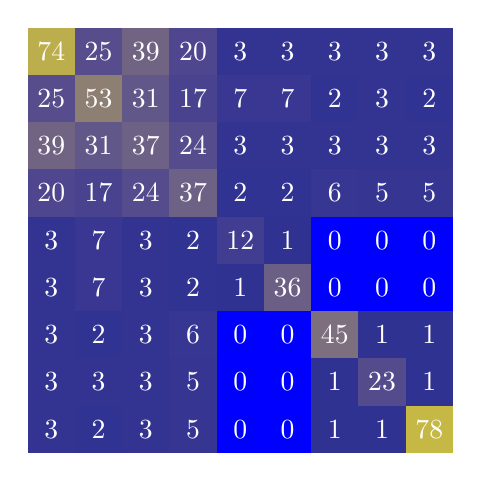
\begin{tikzpicture}[scale=0.6]
  \foreach \y [count=\n] in {
      {74,25,39,20,3,3,3,3,3},
      {25,53,31,17,7,7,2,3,2},
      {39,31,37,24,3,3,3,3,3},
      {20,17,24,37,2,2,6,5,5},
      {3,7,3,2,12,1,0,0,0},
      {3,7,3,2,1,36,0,0,0},
      {3,2,3,6,0,0,45,1,1},
      {3,3,3,5,0,0,1,23,1},
      {3,2,3,5,0,0,1,1,78},
    } {
      \foreach \x [count=\m] in \y {
        \node[fill=yellow!\x!blue, minimum size=6mm, text=white] at (\m,-\n) {\x};
      }
    }
\end{tikzpicture}\quad
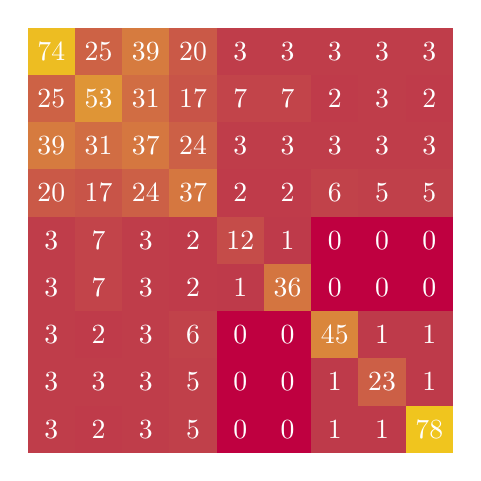
\begin{tikzpicture}[scale=0.6]
  \foreach \y [count=\n] in {
      {74,25,39,20,3,3,3,3,3},
      {25,53,31,17,7,7,2,3,2},
      {39,31,37,24,3,3,3,3,3},
      {20,17,24,37,2,2,6,5,5},
      {3,7,3,2,12,1,0,0,0},
      {3,7,3,2,1,36,0,0,0},
      {3,2,3,6,0,0,45,1,1},
      {3,3,3,5,0,0,1,23,1},
      {3,2,3,5,0,0,1,1,78},
    } {
      \foreach \x [count=\m] in \y {
        \node[fill=yellow!\x!purple, minimum size=6mm, text=white] at (\m,-\n) {\x};
      }
    }
\end{tikzpicture}
}
\caption{图~2的标题名称}
\end{figure}



参考话术:我们需要解决的问题是$\cdots\cdots$,题目要求是$\cdots\cdots$,剔除$\cdots\cdots$数据后选用何种类型的模型优点进行分析。具体步骤123$\cdots$



\subsubsection{***模型的求解}

\textcolor{red}{将预处理数据带入上述模型,通过$\cdots$软件得到$\cdots$结果。(编程代码详见附件*)。模型求解及结果需要图文并茂,用数据说话  用图展示。具体步骤123$\cdots$}
\begin{align}
A_{\max}& =\dfrac{3600}{t_{\min}}=\dfrac{3600}{J_{\min} /(v / 3.6)}
=\dfrac{1000 v}{J_{\min }}(\text{辆 } / h) \\
J_{\min}& =J_{\rm r}+J_{z}+J_{\rm a}
\end{align}


\subsubsection{***结果}

\textcolor{red}{针对于每一个问题的结果综述总结。}



\subsection{问题 三的求解和分析 的求解和分析 的求解和分析}

\subsubsection{对问题的分析}

问题 三要求我们 $\cdots$。

\subsubsection{对问题的求解}

\textbf{模型 Ⅱ—基于 负荷度 负荷度 分析 的小区开放影响度综合评价}

(1)模型的准备

1)负荷度介绍

负荷度( V/CV/CV/C)是指在理想条件下,最大服务交通量与基本行能力之比.

2)数据处理

将道路分为主干和次,其要参数详见 表 10

\begin{table*}[h!]
  \centering
  \small
  \tabcolsep 2.5pt
  \caption{主次道路参数表}
\begin{tabular*}{0.8\linewidth}{p{60pt}<{\centering}p{60pt}<{\centering}
p{60pt}<{\centering}p{80pt}<{\centering}p{80pt}<{\centering}}
\toprule
  道路类型  &  主干路  &  支干路  &  小区内宽道路  &  小区内窄道路  \\
  \midrule
  行车速度  & 50 km / h & 40 km / h & 30 km / h & 20 km / h \\
 车道数  & 4 & 3 & 2 & 1 \\
\bottomrule
  \end{tabular*}
  \label{tab10}
\end{table*}

(2)模型的建立

1)小区的分类

根据小区结构,周边道路分布形状和周边道路车道数的不同,我们将小区分
别分为~4、2、3 类,小区的分类结果详见表~11


2)计算周边各路段及交叉口的通行能力



对于周边各路段的通行能力,我们运用问题二已建立的模型进行计算.在此
基础上对于交叉口的通行能力交叉口~G 我们建立公式如下:

\begin{align}
G_{\text{交又口}}& =\sum_{i=1}^{n} G_{i} \\
G_{i}& =\sum_{j=1}^{k} C_{j}
\end{align}


其中,$C_{j}$ 为进口各车道的通行能力,$ G_{i}$ 为交叉口各进口的通行能力.


3)建立影响度综合评价体系~[9][10][11]

我们采用先单项评价再综合评价的方法,其总体思路见表~12

\begin{table*}[h!]
  \centering
  \small
  \tabcolsep 2.5pt
  \caption{小区分类表}
\begin{tabular*}{0.8\linewidth}{p{100pt}<{\centering}|p{60pt}<{\raggedright}|p{180pt}<{\raggedright}}
\hline
分类标准 & 类型名称& 类型说明\\
\hline
\multirow{4}*{小区结构 }& A组团有序型 & 小区楼房呈组团型分布,每一区域间隔较大,开放后小区
道路较宽,且区域间分布有序\\

& B紧凑有序型 & 小区楼房间隔紧凑,且排列有序,开放后道路网格呈“街
区型”,特点为“高密度、窄路宽.\\
 &C组团无序型& 小区楼房呈组团式分布,每一区域间隔较大,开放后小区
道路较宽,但区域间分布杂乱小区楼房间隔紧凑,但排列杂乱,开放后小区道路呈现“低\\
&D紧凑无序型&密度,窄路宽”的特点\\

\multirow{2}*{周边道路形状分布}& 四周围绕型&四周均为道路\\

&半边包围型&半边围绕道路\\

\multirow{3}*{车道数(针对半封闭性)}& 主干道型 & 两条道路均为主干道\\

&次干道型 & 两条道路均为次干道\\

&混合型& 两条道路一主一次\\
\hline
  \end{tabular*}
  \label{tab11}
\end{table*}

\begin{table*}[h!]
  \centering
  \small
  \tabcolsep 2.5pt
  \caption{综合评价思路表}
\begin{tabular*}{0.8\linewidth}{p{100pt}<{\centering}|p{160pt}<{\raggedright}|p{80pt}<{\raggedright}}
\hline
 评价性质  &  评价内容  &  评价指标  \\
 \hline
\multirow{2}*{ 单项评价 } & \multirow{2}*{  局部路段及交叉口交通负荷影响 } &  路段影响度  \\
& &交叉口影响\\
\multirow{2}*{ 综合评价 } & \multirow{2}*{整个路网交通负荷影响} &平均路段影响度  \\
&&平均交叉口影响度\\
\hline
  \end{tabular*}
  \label{tab12}
\end{table*}

A. 负荷度单项评价

a. 封闭式小区开放后,新增小区内道路对于周边某一路段i 的影响度 $K_{si}$
根据公式计算:
\begin{align}
K_{s i}&=\dfrac{I_{s i p}-I_{s i b}}{B_{s i}} \\
I_{s i p}& =I_{s i b}+a
\end{align}

其中,$I _{sip}$ 为小区道路建成后路段 i 上高峰小时交通量,$I _{sib}$ 为不考虑小区道
 路建成后新增交通量的情况下,路段 i 的高峰小时交通量,  $B_{s i}$  为路段 $i$ 的设计
 通行能力,$a$ 为开放后小区道路的通行量.
b. 封闭式小区开放后,新增小区内道路对于周边道路交叉口的影响度  $K_{c i}$
根据公式计算:
\begin{align}
  K_{c i}=\dfrac{I_{c i p}-I_{c b}}{B_{c t}}
\end{align}


其中,$K_a$ 为小区道路建成后对交叉口 i 的影响度,$I_{crp}$ 为小区道路建成后交 叉口 $i$
上高峰小时交通量, $ I_{c i b}$  为不考虑小区道路建成后新增交通量的情况下, 交叉口 i 的
高峰小时交通量,  $B_{c i}$  为交叉口 $i$ 的设计通行能力.


\begin{figure}[h!t]
\centerline{\includegraphics[scale=1]{fig1.pdf}}
\caption{\song\wuhao 图~3的标题名称}
\end{figure}


\section{模型的评价与推广 模型的评价与推广}

\textcolor{red}{将模型进行数值计算,并与附件中的真实采样值(进行列表或图示)比较。对误差进行数据分析,给出误差分析的理论估计。}

\subsection{模型的评价}


1. 优点

\textcolor{red}{得到满意的解、
较好地解决了$\cdots$问题、
使模型得到简化、
使结果更合理,避免…带来的较大误差、
使问题描述比较清晰、
减少大的计算量。
}

(1)问题求解中 辅之流程图, 将建模思路完整清晰的展现出来;

(2)问题二在对 问题二在对理论通行能力进修复时考虑因素 细致、全面,理论通行能力进修复时考虑因素
 细致、全面,系数准确度高;

(3)在问题三中,提出“影响度”的概念较为直观地定量给小区开放后的效果,简便有.在影响度计算上由
点及面从每个路段、交叉口到整 个路网,层深入具有逻辑性;

\begin{figure}[h!t]
\centerline{\includegraphics[scale=1]{fig4.pdf}}
\caption{\song\wuhao 图~3的标题名称}
\end{figure}


(4)运用多种数学软件(如 MATLAB、SPSS),取长补短,使计算结果更加),取长补短,使计算结果更
加 准确、明晰.

2. 缺点

\textcolor{red}{主观性过强、
建立在什么的前提条件下、
有一定的局限性、
存在不确定性、
有一定的偏差。
}

(1)在数学软件的计算中会将小数计算 结果进行保留,使得随后的会将小数计算 结果进行保留,使得随后
的或统计结果造成一定误差;

(2)问题二求解修正通行能力时多次使用了查表,操作不够简便.

\subsection{模型的、模型的 推广}

\begin{itemize}

\item \textcolor{red}{对本文中的模型给出比较客观的评价,必须实事求是,有根据,以便评卷人参考。}

\item \textcolor{red}{推广和优化,需要花费功夫想出合理的、甚至可以合理改变题目给出的条件的、不一定可行但是具有一定想象空间的准理想的方法、模型。由此做出一些改进方向,也可以是参赛者一些来不及实现的思路。}
\end{itemize}

1. 问题二中 建立 的模型 在现实 生活 中可以 作为 检验 数据 对实测数据 的准确 性进行 检验,帮助 人们
更好 的测算 交通 数据.

2. 基于问题三建立的模型,可以根据道路实时检测数(某段单位间内 基于问题三建立的模型,推算新建
一条道路对于当前交 通状况的改善效果,帮助度等).

\section{模型的改进}

\subsection{模型一的改进}
针对问题二中的模型一,在具体求解大型车对车辆通行能力的修正系数时,
我们利用交通量的测算值对照得到相应的大型车修正系数.但是,在实际操作中
交通量的测定有很大的难度,如果此时交通量数据无法得到,那么我们便不能得
到相应的修正系数,因此我们对模型进行改进.

由~GREENSHIELD K-V 线性模型,可得通行能力的公式:
\begin{align}
A_{p}=\begin{cases}
\dfrac{3600}{t}\left(1-\dfrac{3.6 l}{V_{t} t}\right)\left(V_{f}>7.2 l / t\right) \\
\dfrac{250 V_{f}}{t}\left(V_{f} \leq 7.2 l / t\right)
\end{cases}
\end{align}

对应的临界车辆速度:
\begin{align}
V_{p}=\begin{cases}
\dfrac{V_{f}-3.6 l}{t} & \left(V_{f}>7.2 l / t\right) \\
\dfrac{1}{2} V_{f} & \left(V_{f} \leq 7.2 l / t\right)
\end{cases}
\end{align}

由美国道路通行能力准则可得,美国将道路服务水平分为六级:A-F 级,而
我国目前针对当前国情,将道路服务水平分成四级:一级相当于美国的A、B 两
级;二级相当于美国的C 级;三级相当于美国的D 级;四级相当于美国的E、F
级。因此,相应的,将美国服务水平划分标准进行针对性修正,得到中国道路服
务水平划分标准,见表

\begin{table*}[h!]
  \centering
  \small
  \tabcolsep 2pt
  \caption{我国服务水平划分标准}
\begin{tabular*}{0.87\linewidth}{p{60pt}<{\centering}p{40pt}<{\centering}
p{40pt}<{\centering}p{40pt}<{\centering}p{40pt}<{\centering}
p{80pt}<{\centering}p{40pt}<{\centering}}
\toprule
服务水平 (L0S)  & \multicolumn{2}{c} {一级 } & 二级  & 三级  & \multicolumn{2}{c} {四级 } \\
\cline{2-3}\cline{6-7}
服务交通量  & 800 & 1200 & 1800 & 2500 & $A_{D}$ & $\leqslant A_{P}$ \\
 速度  km / h & 120 & 120 & 120 & 120 & $\geqslant V_{p}$ & $\leqslant V_{p}$ \\
 V / C & 0.33 & 0.48 & 0.71 & 1.0 & $A_{p} / A_{\max}\leqslant 1.0$ & -(无意义 ) \\
\bottomrule
  \end{tabular*}
\end{table*}

由于车流量的测算相对于交通量来说较易得到,我们便可以不用对交通量进
行测算,可以通过车流量与通行能力的比值计算出~V/C 饱和度值,再通过该值对
照我国服务水平划分标准,间接得到服务交通量,从而得到大型车对通行能力的
修正系数.


\subsection{模型二的改进}

针对于问题三中的模型,在得出各个类型小区在开放后对于整个小区周边路
网交通负荷影响度后,无法判别小区开放的效果是积极的还是消极的,由此我们
可以采用~Bress 悖论的原理进行判别:在个人独立选择路径的情况下,为某路网
增加额外的通行能力(如增加路段的等),反而会导致整个路网的整体运行水平
降低的情况.

将路网进行简化如图~15:

根据推导可得: 当 $\beta_{3}/\left(\beta_{1}+\beta_{2}\right) \leq\left(\beta_{5}+\beta_{6}\right)/\beta_{4}$ 时,会发生悖论,即道路的开
通反而会加剧原有道路的交通状况.

\textcolor{red}{需重新起页,不得与论文正文内容在同一页上}

\begin{rmk}
5篇以上!
\end{rmk}

\newpage

\begin{thebibliography}{99}
\addcontentsline{toc}{section}{参考文献}
\bibitem{1} 李向鹏. 城市交通拥堵对策——封闭型小区交通开放研究~[D]. 交通运输工程,
2014.4.
\bibitem{2} 司守奎等. 数学建模算法与应用~[M]. 北京:国防工业出版社,2011.8 第一版;
\bibitem{3} 吕彬. 城市居住区“开放性”模式研究~[D]. 建筑设计,2006.6.
\bibitem{4} 茹红蕾. 城市道路通行能力的影响因素研究~[D]. 交通运输工程,2008.3.
\bibitem{5} VISSIM 软件路网搭建教程.
http://wenku. baidu.com/view/7bc33214680203d8ce2f24c4.html
\bibitem{6} 赵琳,邵长桥. 基于~VISSIM 的高速公路基本路段实际通行能力仿真分析~[J]. 道
路交通与安全,2007.2.
\bibitem{7} 李冬梅,李文权. 道路通行能力的计算方法 [J]. 河南大学学报,2002.6:24-27.
\bibitem{8} 城市轨道施工安全及交通组织 [S].2014.
\bibitem{9} 李鑫, 李雪等. 城市道路网络脆弱性评估指标研究综述~[J]. 公路交通科技,
2016.1:155-157.
\bibitem{10} 詹斌, 蔡瑞东等. 基于城市道路网络脆弱性的小区开放策略研究 [J]. 技术方法,
2016.7:98-101.
\bibitem{11} 彭驰. 物流园区交通影响分析研究~[D]. 交通运输工程,2007, 4.

\end{thebibliography}
\newpage

\begin{appendices}

\section*{}

\textbf{\textcolor[rgb]{0.98,0.00,0.00}{程序一:MATLAB算道路车辆通行能力:}}
\lstinputlisting[language=Matlab]{./code/mcmthesis-matlab1.m}

\section*{}

\textcolor[rgb]{0.98,0.00,0.00}{\textbf{程序二:C++ 求解路网正体影响度:}}
\lstinputlisting[language=C++]{./code/mcmthesis-sudoku.cpp}

\newpage
\def\thesection{A}
\renewcommand{\thetable}{\wuhao A-\arabic{table}}
\setcounter{table}{0}
\section*{数据表格}
\textcolor[rgb]{0.98,0.00,0.00}{\textbf{表格数据:}}
\input{Appendices1}

\end{appendices}
\end{document}
%%
%% This work consists of these files mcmthesis.dtx,
%%                                   figures/ and
%%                                   code/,
%% and the derived files             mcmthesis.cls,
%%                                   mcmthesis-demo.tex,
%%                                   README,
%%                                   LICENSE,
%%                                   mcmthesis.pdf and
%%                                   mcmthesis-demo.pdf.
%%
%% End of file `mcmthesis-demo.tex'.
